%\section{$A^*$ Greedy Algorithm} \label{sec:krd_greedy}
\section{Discovery Algorithm} \label{sec:krd_greedy}
We introduce a greedy approach to solve the approximate version of the discovery problem (Section~\ref{sec:krd_prob_def}). The algorithm combines two phases:
\begin{inparaenum}[\itshape(i)]
	\item it solves the set cover problem with a greedy strategy;
	\item it discovers new rules by navigating the graph in the $A^*$ search fashion.
	%, allowing the pruning of unpromising paths.	
\end{inparaenum}

\vspace{-1ex}
\subsection{Marginal Weight}
\vspace{-0.2ex}
%In Section~\ref{sec:krd_weight_fun}, we defined the weight associated with a set of rules $R$ with two components that model the role of positive and negative examples, respectively.
%as follows:
%\begin{equation*}
%w(R) = \alpha \cdot (1-\frac{\mid C_{R}(G)\mid}{\mid G \mid}) +\beta \cdot (\frac{\mid C_{R}(V) \mid}{\mid U_{R}(V)\mid})
%\end{equation*}
%Our goal is to discover a set of rules that covers as many elements as possible in $G$, and as few elements as possible in $V$. 
We follow the intuitions behind the greedy algorithm for weighted set cover by defining a \emph{marginal weight} for rules that are not yet included in the solution~\cite{chvatal1979greedy}.

\begin{definition}
\label{def:marweight}
	Given a set of rules $R$ and a rule $r$ such that $r \notin R$, the marginal weight of $r$ w.r.t. $R$ is defined as:
	\begin{equation*} \label{eq:mar_weight}
	w_m(r) = w(R \cup \{r\}) - w(R) 
	%- \alpha \cdot \frac{\mid C_{r}(G) \setminus C_{R}(G) \mid}{\mid G \mid} + \beta \cdot (\frac{\mid C_{R \cup \{r\}}(V) \mid}{\mid U_{R \cup \{r\}}(V) \mid} - \frac{\mid C_{R}(V) \mid}{\mid U_{R}(V) \mid})
		\vspace{-0.5ex}
	\end{equation*}
\end{definition}

The marginal weight quantifies the %total 
weight increase by adding $r$ to an existing set of rules. % $R$. 
%%%JOURNAL% In other words, it indicates the contribution of $r$ to $R$ in terms of new elements covered in $G$ and new elements unbounded covered in $V$. 
%Due to the first negative part of the marginal weight, $w_m(r) \in [-\alpha,+\beta]$. 
Since the %set cover 
problem aims at minimizing the total weight, we never add a rule to the solution if its marginal weight is greater than or equal to $0$.

%%!TEX root = ../cleaning-vldb-16.tex
{\singlespacing
  \begin{algorithm}[t]\small
      \SetKwInOut{Input}{input}
      \SetKwInOut{Output}{output}
      
      \SetKwFunction{sinInRule}{singleInstanceRule}
      
	
      \SetKwData{mannot}{$\mathcal{M}_{annot}$}
	
      \Input{$G$ -- generation set}
      \Input{$V$ -- validation set}
      \Input{$R$ -- universe of rules}
      \Output{$R_{opt}$ -- greedy set cover solution}
      
      	$R_{opt} \gets \emptyset$\;
      	$r \gets \underset{w_m(r)}{\operatorname{argmin}}(r \in R)$\;
      	\Repeat{$R = \emptyset \vee C_{R_{opt}}(G) = G \vee w_m(r) \geq 0$}
      	{
      		$R_{opt} \gets R_{opt} \cup \{r\}$\;
      		$R \gets R \setminus \{r\}$\;
      		$r \gets \underset{w_m(r)}{\operatorname{argmin}}(r \in R)$\;
      	}
      	\If{$C_{R_{opt}}(G) \neq G$}{
      		$R_{opt} \gets R_{opt} \cup \sinInRule(G \setminus C_{R_{opt}}(G))$\;
      		
      	}
  
  \Return{$R_{opt}$}
  \caption{Greedy Rules Selection.}
  \label{alg:krd_greedy}
  \end{algorithm}
}

%Algorithm~\ref{alg:krd_greedy} shows the straightforward 
%In the greedy rule selection procedure. 
The algorithm for greedy rule selection is then straightforward:
given a generation set $G$, a validation set $V$, and the universe of all possible rules $R$, the algorithm picks at each iteration the rule $r$ with minimum marginal weight and add it to the solution $R'$. % $R_{opt}$.
%takes as input the generation set $G$, the validation set $V$, and the universe of all possible rules $R$. The set of output rules $R_{opt}$ is first assigned to an empty set. At each iteration, the algorithm picks from $R$ the rule $r$ with the minimum marginal weight, and it adds $r$ to $R_{opt}$, $r$ is then removed from $R$. 
The algorithm stops when one of the following termination conditions is met:
\begin{inparaenum} [\itshape1)]
	\item $R$ is empty -- all the rules have been included in the solution;
	\item $R'$ covers all elements of $G$;
	\item the minimum marginal weight is greater than or equal to $0$, i.e., among the remaining rules in $R$, none of them has a negative marginal weight.
	%, hence the current solution is the one with the minimum weight.
\end{inparaenum}
%WE CAN ELIMINATE THE NEXT SENTENCE IF WE NEED SPACE
%%%JOURNAL% The marginal weight is greater than or equal to $0$ whenever (i) the rule does not cover new elements in $G$, and (ii) it does not unbounded cover new elements in $V$. 
%%%JOURNAL% If the second termination condition is not met, there may exist examples in $G$ that are not covered by $R_{opt}$. In such a case the algorithm will augment $R_{opt}$ with single-instance rules (rules that cover only one example), one for each element in $G$ not covered by $R_{opt}$.
%WILL? do we do it? <<<<<<<<

%Since the coverage of a rule is always contained in its unbounded coverage, 
%UNBOUND COVER? then below should be unbound covered, i guess <<<
%More specifically, a rule $r$ has a negative marginal weight iff the sum of its new elements covered in $G$ with its new elements unbounded covered in $V$ is strictly greater than its new elements covered in $V$ multiplied by some $\gamma$, where $\gamma$ depends on how we set $\alpha$ and $\beta$.

The greedy solution guarantees a \texttt{log($k$)} approximation
to the optimal solution~\cite{chvatal1979greedy}, where $k$ is the largest number of elements covered in $G$ by a rule in $R$.
%%%JOURNAL% and $k$ is at most $|G|$. 
If the optimal solution is made of 
%output rules in the final solution cover 
rules that cover disjoint sets over $G$, then the greedy solution coincides with the optimal one.

\vspace{-1ex}
\subsection{$A^*$ Graph Traversal}
\vspace{-0.2ex}
The greedy algorithm for weighted set cover assumes that the universe of rules $R$ has been generated.
%, so that we can iteratively pick the rule with minimum marginal weight. 
To generate $R$, we need to traverse all valid paths from a node $x$ to a node $y$, for every pair $(x,y) \in G$. But do we need all possible paths for every example? % in $G$?
	%	\vspace{-1.5ex}

	\begin{figure}%[htb]
		\centering
		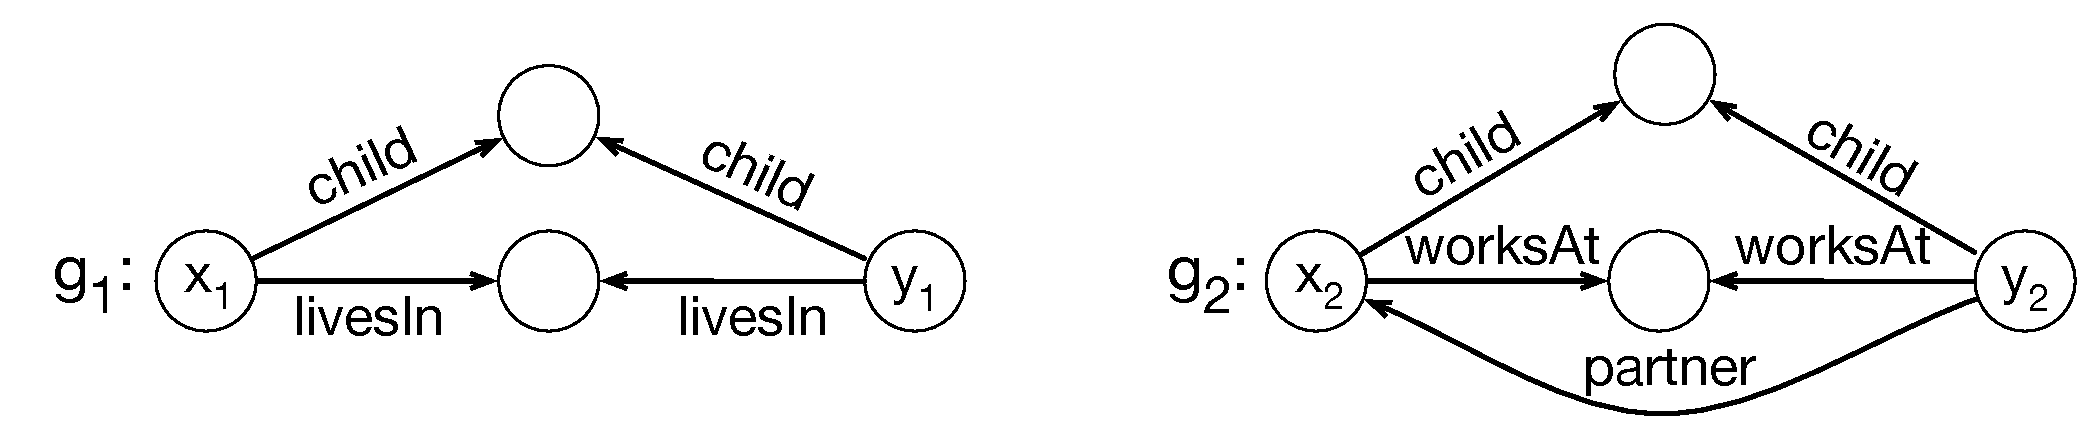
\includegraphics[width=0.99\columnwidth]{include/figure/a*_graph_example.pdf}	
		\vspace{-2.5ex}
		\caption{Two positive examples.}
	\label{fig:positive_examples}
		\vspace{-1.5ex}
\end{figure}

\begin{example}
	Consider the mining of positive rules for the target predicate \texttt{spouse}. The generation set $G$ includes two examples $g_1$ and $g_2$ shown as graphs in Figure~\ref{fig:positive_examples}. % shows the corresponding KB graphs. % for the two examples. 
	Assume for simplicity that all rules in the universe have the same coverage and unbounded coverage over the validation set $V$.
	One candidate rule is $r : \atom{child}{x}{v_0} \wedge \atom{child}{y}{v_0} \Rightarrow \atom{spouse}{x}{y}$, stating that entities $x$ and $y$ with a common child are married. %Looking at the KB 
	In the graph, $r$ covers both $g_1$ and $g_2$.
	%-- in both $g_1$ and $g_2$ there exists a path that corresponds to $r_{body}$. 
	Since all rules have the same coverage and unbounded coverage over $V$, 
	%if we include $r$ in the solution, %before inspecting other potential rules, then 
	there is no need to generate any other rule. In fact, any other candidate rule will not cover new elements in $G$, therefore their marginal weights will be greater than or equal to $0$. 
	%Hence any other rule will not be part of the solution. 
	Thus the creation and navigation of edges \texttt{livesIn} in $g_1$, \texttt{worksAt} in $g_2$, and \texttt{partner} in $g_2$ is not needed.
\end{example}

Based on the above observation, we avoid the generation of the entire universe $R$, but rather consider at each iteration the most promising path on the graph. The same intuition  is behind 
the $A^*$ graph traversal algorithm~\cite{hart1968formal}. 
%%%JOURNAL%Given an input weighted graph, $A^*$ computes the smallest cost path from a starting node $s$ to an ending node $t$. At each iteration, $A^*$ maintains a queue of partial paths starting from $s$, and it expands one of these paths based on an \emph{estimation} of the cost to reach $t$. The path with the best estimation is expanded and added to the paths queue. The algorithm keeps iterating until one of the partial paths reaches $t$. 
%%%JOURNAL%
%%%JOURNAL%We discover rules with a similar technique. 
For each example $(x,y) \in G$, we start the navigation from $x$. We keep a queue of not valid rules, 
%%%JOURNAL%(Section~\ref{sec:krd_language}), 
and at each iteration we consider the rule with the minimum marginal weight, which corresponds to paths in the example graphs. 
We expand the rule by following the edges, and we add the new founded rules to the queue of not valid rules. Unlike $A^*$, we do not stop when a rule (path) reaches the node $y$ (i.e., becomes valid). Whenever a rule becomes valid, we add the rule to the solution and we do not expand it any further. The algorithm keeps looking for plausible paths until one of the termination conditions of the greedy cover algorithm is met. %Algorithm~\ref{alg:krd_greedy} is met.

A crucial point in $A^*$ is the definition of the estimation cost. To guarantee the solution to be optimal, the estimation must be \emph{admissible}~\cite{hart1968formal}, i.e., the estimated cost must be less than or equal to the actual cost. 
%%%JOURNAL% For example, for the shortest route problem, an admissible estimation is the straight-line distance to the goal for every node, as it is physically the smallest distance between any two points. 
In our setting, given a rule that is not yet valid and needs to be expanded, we define an admissible estimation of the marginal weight.

\begin{definition}
	Given a rule $r : A_1 \wedge A_2 \cdots A_n \Rightarrow B$, we say that a rule $r'$ is an \emph{expansion} of $r$ iff $r'$ has the form $A_1 \wedge A_2 \cdots A_n \wedge A_{n+1} \Rightarrow B$. %In other words, $r'$ is generated by adding a new atom to the body of $r$.
\end{definition}
%WE ALREADY USED expand MULTIPLE TIMES ABOVE. Should this go earlier? is it needed? <<<<

%In other words, Expanding $r$ means adding a new atom to its body. 
In the graph traversal, expanding $r$ means traversing one further edge on the path defined by $r_{body}$. To guarantee the optimality condition, the estimated marginal weight for a rule $r$ that is not valid must be less than or equal to the actual weight of any valid rule that is generated by expanding $r$. Given a rule and some expansions of it, we can derive the following.

\begin{lemma} \label{lemma:krd_exp_cov}
	Given a rule $r$ and a set of pair of entities $E$, then for each $r'$ expansion of $r$, $C_{r'}(E) \subseteq C_r(E)$ and $U_{r'}(E) \subseteq U_r(E)$.
\end{lemma}


The above Lemma states that the coverage and unbounded coverage of an expansion $r'$ of $r$ are contained in the coverage and unbounded coverage of $r$, respectively, and directly derives from the augmentation inference rule for functional dependencies~\cite{abiteboul1995foundations}. 
%In fact, expanding a rule with a new atom to its body makes the rule more selective. 
%This is equivalent of adding an `AND' condition to a SQL query $q$: the new result will obviously be a subset of the result obtained with $q$.
%Note that Lemma~\ref{lemma:krd_exp_cov} is equivalent to the 

%We recall that the merginal weight of a rule $r$ w.r.t. a solution $R$ is defined as follow:
%\begin{equation*}
%w_m(r) = - \alpha \cdot \frac{\mid C_{r}(G) \setminus C_{R}(G) \mid}{\mid G \mid} + \beta \cdot (\frac{\mid C_{R \cup \{r\}}(V) \mid}{\mid U_{R \cup \{r\}}(V) \mid} - \frac{\mid C_{R}(V) \mid}{\mid U_{R}(V) \mid})
%\end{equation*}
The only positive contribution to marginal weights is given by $|C_{R \cup \{r\}}(V)|$. $|C_{R \cup \{r\}}(V)|$ is equivalent to $|C_{R}(V)| + |C_r(V) \setminus C_R(V)|$, thus if we set $|C_r(V) \setminus C_R(V)|=0$ for any $r$ that is not valid, we guarantee an admissible estimation of the marginal weight. We estimate the coverage over the validation set to be $0$ for any rule that can be further expanded, since expanding it may bring the coverage to $0$.
%CANNOT NOT NOTICE HOW BRUTAL IT"S THIS ESTIMATE!

\begin{definition}\label{def:est_res_wei}
	Given a \emph{not valid} rule $r$ and a set of rules $R$, we define the \emph{estimated marginal weight} of $r$ as:
	\begin{equation*}
	w_m^*(r) = - \alpha \cdot \frac{\mid \hspace{-0.5ex} C_{r}(G) \setminus C_{R}(G) \hspace{-0.5ex} \mid}{\mid \hspace{-0.5ex} G \hspace{-0.5ex} \mid} + \beta \cdot (\frac{\mid \hspace{-0.5ex} C_R(V) \hspace{-0.5ex} \mid}{\mid \hspace{-0.5ex} U_{R \cup \{r\}}(V) \hspace{-0.5ex} \mid} - \frac{\mid \hspace{-0.5ex} C_{R}(V) \hspace{-0.5ex} \mid}{\mid \hspace{-0.5ex} U_{R}(V) \hspace{-0.5ex} \mid})
	\end{equation*}
	%where a rule is valid iff it respects the language biases defined in Section~\ref{sec:krd_language}.
\end{definition}
%I AM A BIT CONFUSED BY THE FORMULA, i was expecting a 0 in the first case <<<<<

The estimated marginal weight for a valid rule is equal to the actual marginal weight from Definition~\ref{def:marweight}.
%defined in Equation~\ref{eq:mar_weight}. 
Valid rules are not considered for expansion, therefore we do not need to estimate their weights since we know the actual ones. Given Lemma~\ref{lemma:krd_exp_cov}, we can easily see that $w_m^*(r) \leq w_m^*(r')$, for any $r'$ expansion of $r$. Thus our marginal weight estimation is admissible. 
%Due to the first negative part of the marginal weight, $w_m^*(r) \in [-\alpha,+\beta]$. 



%to remove vertical space after algorithm
\setlength{\textfloatsep}{0pt}% Remove \textfloatsep
{\singlespacing
  \begin{algorithm}[t]\small
      \SetKwInOut{Input}{input}
      \SetKwInOut{Output}{output}
      
      \SetKwFunction{expFron}{expandFrontiers}
      \SetKwFunction{frontiers}{frontiers}
      \SetKwFunction{isValid}{isValid}
      \SetKwFunction{length}{length}
      \SetKwFunction{sinInRule}{singleInstanceRule}
      
	
      \SetKwData{mannot}{$\mathcal{M}_{annot}$}
	
      \Input{$G$ -- generation set}
      \Input{$V$ -- validation set}
      \Input{$maxPathLen$ -- maximum rule body length}
      \Output{$R_{opt}$ -- greedy set cover solution}
      
      	$R_{opt} \gets \emptyset$\;
      	$N_f \gets \{x | (x,y) \in G\}$\; \label{alg_line:front_nodes}
      	$Q_r \gets \expFron(N_f)$\; \label{alg_line:sparql_1}
      	%$\quad$\tcp{SPARQL}%
      	$r \gets \underset{w_m^*(r)}{\operatorname{argmin}}(r \in Q_r)$\; \label{alg_line:q_r_initialisation}
      	\Repeat{$Q_r = \emptyset \vee C_{R_{opt}}(G) = G \vee w_m^*(r) \geq 0$}
      	{
      		$Q_r \gets Q_r \setminus \{r\}$\;
      		\If{$\isValid(r)$}{
      			$R_{opt} \gets R_{opt} \cup \{r\}$\; \label{alg_line:valid_rule}
      		}
      		\Else{
      			\tcp{rules expansion}
      			\If{$\length(r_{body}) < maxPathLen$ \label{alg_line:exp_condition}}
      			{
      				$N_f \gets \frontiers(r)$\;
      				$Q_r \gets Q_r \cup \expFron(N_f)$\;  \label{alg_line:sparql_2}
	      			%$\quad$\tcp{SPARQL}
      			}
      		}
      		$r \gets \underset{w_m^*(r)}{\operatorname{argmin}}(r \in Q_r)$\;
      	}
      	\If{$C_{R_{opt}}(G) \neq G$}{
      		$R_{opt} \gets R_{opt} \cup \sinInRule(G \setminus C_{R_{opt}}(G))$\;
      		
      	}
  
  \Return{$R_{opt}$}
  \caption{\krd Rule Discovery.}
  \label{alg:krd_a*}
  \end{algorithm}
}
\vspace{-2ex}
%restablish some space
\setlength{\textfloatsep}{5pt}

We are ready to introduce Algorithm~\ref{alg:krd_a*}, which shows the modified set cover procedure, including the $A^*$-like rule generation.
For a rule $r$, we call \emph{frontier nodes}, $N_f(r)$, the last visited nodes in the paths that correspond to $r_{body}$ from every example graphs covered by $r$. 
%%%%JOURNAL%% As an example, given $r_{body} = \atom{child}{x}{v_0}$, $N_f(r)$ contains all the entities $v_0$ that are children of $x$, for every $(x,y) \in G$. 
%-- $v_0$ is the last visited node in the path. 
Expanding a rule $r$ implies navigating a single edge from any frontier node. In the algorithm, the set of frontier nodes is initialized with starting nodes $x$, for every $(x,y) \in G$ (Line~\ref{alg_line:front_nodes}). The algorithm maintains a queue of rules $Q_r$, from which it chooses at each iteration the rule with minimum estimated weight. 
The function \texttt{expandFrontiers} retrieves %%%%JOURNAL%%from the KB 
all nodes (along with edges) at distance $1$ from frontier nodes and returns the set of all rules generated by this one hop expansion. 
%%%%JOURNAL%% Such expansions are computed with single-hop SPARQL queries. 
$Q_r$ is therefore initialized with all rules of length $1$ starting at $x$ (Line~\ref{alg_line:sparql_1}). In the main loop, the algorithm checks if the current best rule $r$ is valid or not. If $r$ is valid, it is added to the output and it is not expanded (Line~\ref{alg_line:valid_rule}). If $r$ is not valid, it is expanded iff the length of its body is less than $maxPathLen$ (Line~\ref{alg_line:exp_condition}). 
%Rules with body greater than or equal to $maxPathLen$ are not expanded as they are not allowed in the output. 
The termination conditions and the last part of the algorithm are the same of the %%%%JOURNAL%%previously described 
greedy set-cover algorithm. % Algorithm~\ref{alg:krd_greedy}.

The simultaneous rule generation and selection of Algorithm~\ref{alg:krd_a*} brings multiple benefits. First, we do not generate the entire graph for every example in $G$. Nodes and edges are generated \emph{on demand}, whenever the algorithm requires their navigation (Line~\ref{alg_line:sparql_2}). 
%%%%JOURNAL%% If the initial part of a path is not promising according to its estimated weight, the rest of the path will never be materialized. % since there is no need to navigate it. 
%Materializing the graph is an expensive task, since we need to query the disk to retrieve target nodes and edges. 
Rather than materializing the entire graph and then traversing it, our solution gradually materializes parts of the graph whenever they are needed for navigation (Lines~\ref{alg_line:sparql_1} and~\ref{alg_line:sparql_2}). 
Second, the weight estimation leads to pruning unpromising rules. If a rule does not cover new elements in $G$ and does not unbounded cover new elements in $V$, then it %%%%JOURNAL%%s estimated marginal weight is $0$ and 
will be pruned. 
%A rule with $0$ marginal weight is never picked for expansion.
%A BIT PUZZLED, we have tons of rules with estimated marginal weight, no? <<<<<<<<
%, and if it is the algorithm terminates (due to one of the termination conditions). This implies that a rule with $0$ estimated marginal weight is pruned away from the search space, as we will never generate rules from its expansion.

%FOLLOWING PARAGRAPH REMOVED for the sake of SPACE. TO BE RECYCLED somewhere else?? <<<<<
%The partial materialization of the graph and the pruning of the search space have a significant impact on the algorithm's resources. The running time is halved in the worst case and ten times faster in the best one. We also significantly decrease the amount of memory needed, since we load sub-portions of the graph. Consider the extreme case where there exists a rule $r$ that covers all elements in $G$, unbound covers all elements in $V$ and does not cover any element of $V$. In such a case, Algorithm~\ref{alg:krd_a*} will output the optimal solution by just materialising paths on the example graphs that correspond to $r_{body}$ with $\bigO{l \cdot |G|}$ SPARQL queries, where $l$ is the length of $r_{body}$.





